\documentclass[10pt,letterpaper]{article}
\usepackage[top=0.85in,left=2.75in,footskip=0.75in,marginparwidth=2in]{geometry}

% use Unicode characters - try changing the option if you run into troubles with special characters (e.g. umlauts)
\usepackage[utf8]{inputenc}

% clean citations
\usepackage{cite}

% hyperref makes references clicky. use \url{www.example.com} or \href{www.example.com}{description} to add a clicky url
\usepackage{nameref,hyperref}

% line numbers
\usepackage[right]{lineno}

% improves typesetting in LaTeX
\usepackage{microtype}
\DisableLigatures[f]{encoding = *, family = * }

% text layout - change as needed
\raggedright
\setlength{\parindent}{0.5cm}
\textwidth 5.25in 
\textheight 8.75in

% Remove % for double line spacing
%\usepackage{setspace} 
%\doublespacing

% use adjustwidth environment to exceed text width (see examples in text)
\usepackage{changepage}

% adjust caption style
\usepackage[aboveskip=1pt,labelfont=bf,labelsep=period,singlelinecheck=off]{caption}

% remove brackets from references
\makeatletter
\renewcommand{\@biblabel}[1]{\quad#1.}
\makeatother

% headrule, footrule and page numbers
\usepackage{lastpage,fancyhdr,graphicx}
\usepackage{epstopdf}
\pagestyle{myheadings}
\pagestyle{fancy}
\fancyhf{}
\rfoot{\thepage/\pageref{LastPage}}
\renewcommand{\footrule}{\hrule height 2pt \vspace{2mm}}
\fancyheadoffset[L]{2.25in}
\fancyfootoffset[L]{2.25in}

% use \textcolor{color}{text} for colored text (e.g. highlight to-do areas)
\usepackage{color}

% define custom colors (this one is for figure captions)
\definecolor{Gray}{gray}{.25}

% this is required to include graphics
\usepackage{graphicx}

% use if you want to put caption to the side of the figure - see example in text
\usepackage{sidecap}

% use for have text wrap around figures
\usepackage{wrapfig}
\usepackage[pscoord]{eso-pic}
\usepackage[fulladjust]{marginnote}
\reversemarginpar

% Adding multirow.
\usepackage{multirow}

% Other required things:
\usepackage{color}
\usepackage{subcaption}
\captionsetup[subfigure]{justification=centering}
\newcommand{\beachmat}{\textit{beachmat}}
\newcommand{\code}[1]{\texttt{#1}}

\newcommand{\suppfigsimpleaccess}{1}
\newcommand{\suppfigsparseschem}{2}
\newcommand{\suppfigsparsecol}{3}
\newcommand{\suppfigsparserow}{4}
\newcommand{\suppfighdfspeed}{5}
\newcommand{\suppfighdflayout}{6-7}

\newcommand{\suppsecsimple}{1.1}
\newcommand{\suppsecsparse}{1.2}
\newcommand{\suppsechdfmat}{1.3}
\newcommand{\suppsecother}{1.4}
\newcommand{\suppseclayoutoptim}{2}
\newcommand{\suppseclayouttest}{3}

% document begins here
\begin{document}
\vspace*{0.35in}

% title goes here:
\begin{flushleft}
{\Large
    \textbf\newline{beachmat: a Bioconductor C++ API for accessing single-cell genomics data from a variety of R matrix types}
}
\newline

% authors go here:
%\\
Aaron T. L. Lun\textsuperscript{1,*},
Herv\'e Pag\`es\textsuperscript{2},
Mike L. Smith\textsuperscript{3}
\\
\bigskip
\bf{1} Cancer Research UK Cambridge Institute, University of Cambridge, Li Ka Shing Centre, Robinson Way, Cambridge CB2 0RE, United Kingdom \\
\bf{2} Fred Hutchinson Cancer Research Center, 1100 Fairview Ave N, Seattle, WA 98109, USA \\
\bf{3} European Molecular Biology Laboratory (EMBL), Genome Biology Unit, 69117 Heidelberg, Germany
\\
\bigskip
* aaron.lun@cruk.cam.ac.uk

\end{flushleft}

\section*{Abstract}
Recent advances in single-cell RNA sequencing have dramatically increased the number of cells that can be profiled in a single experiment.
This provides unparalleled resolution to study cellular heterogeneity within biological processes such as differentiation.
However, the explosion of data that are generated from such experiments poses a challenge to the existing computational infrastructure for statistical data analysis.
In particular, large matrices holding expression values for each gene in each cell require sparse or file-backed representations for manipulation with the popular R programming language.
These alternative representations are not easily compatible with high-performance C++ code used for computationally intensive tasks in existing R packages.
Here, we describe a C++ interface named \beachmat{}, which enables agnostic data access from various matrix representations.
This allows package developers to write efficient C++ code that is interoperable with simple, sparse and HDF5-backed matrices, amongst others.
We perform simulations to examine the performance of \beachmat{} on each matrix representation, 
and we demonstrate how \beachmat{} can be incorporated into the code of other packages to drive analyses of a very large single-cell data set.

% now start line numbers
\linenumbers

\section*{Introduction}
Recent advances in single-cell RNA sequencing (scRNA-seq) technologies have led to an explosion in the quantity of data that can be generated in routine experiments.
Droplet-based methods such as Drop-Seq \cite{macosko2015highly}, inDrop \cite{klein2015droplet} and GemCode \cite{zheng2017massively} allow transcriptome-wide expression profiles involving 10,000-40,000 genes to be captured in each of thousands to millions of cells.
Careful computational analysis is critical to extract meaningful biology from these data, but their sheer volume strains existing pipelines and methods designed for single-cell data processing.
The data analysis challenge is compounded by the presence of large-scale projects such as the Human Cell Atlas \cite{regev2017human}, which aims to use single-cell `omics to profile every cell type in the human body.
Similar issues are encountered outside of transcriptomics, with single-cell ATAC-seq \cite{buenrostro2015single} and bisulfite sequencing \cite{smallwood2014single} providing region- to base-level resolution of biochemical events (chromatin accessibility and DNA methylation, respectively).

The statistical programming language R \cite{R} is a key platform for processing and exploring scRNA-seq data sets.
R provides efficient, rigorously tested, open-source implementations of many statistical and numerical procedures.
Its interactive nature lends itself to data exploration and research, while its programming features allow assembly of complex analyses.
It is also extensible through the installation of optional ``packages", often contributed by the research community, which contain bespoke methods for specific scientific problems.
In particular, the Bioconductor project \cite{gentleman2004bioconductor,huber2015orchestrating} provides packages for biological data analysis, many of which implement established methods for single-cell `omics data analysis \cite{trapnell2014dynamics,lun2016pooling,mccarthy2017scater,finak2015mast}
Packages are mostly written in R but can also include native code (in C/C++ or Fortran) for computationally intensive tasks.
Use of native C++ code is facilitated by the \textit{Rcpp} package \cite{eddelbuettel2011seamless}, which simplifies the integration of package code with the R application programming interface (API).

In its simplest form, a scRNA-seq data set consists of a matrix where each column is a cell, each row is a gene, and the value of each matrix entry is set to the quantified expression (e.g., number of mapped reads, transcripts-per-million) for that gene in that cell.
This is most directly represented in R as a simple matrix, where each entry is explicitly stored in memory in a dense contiguous array.
Alternatively, it can be represented as a sparse matrix using classes from the \textit{Matrix} package \cite{bates2017matrix}, which saves memory by only storing non-zero entries.
This exploits the low capture efficiencies of current scRNA-seq protocols \cite{grun2015design} that are responsible for the high frequency of zeroes in the data.
Another option is to use file-backed representations such as those in the \textit{bigmemory} \cite{kane2013scalable} or \textit{HDF5Array} packages, where the data are stored on disk and parts of it are loaded into memory upon request.
In each case, methods are provided in R for common operations such as subsetting, transposition and arithmetic, such that any downstream code for data processing can be agnostic to the exact representation of the matrix.
This simplifies software development and improves interoperability.

Unfortunately, for native code written in statically typed languages like C++, the details of the matrix representation must be known during compilation.
This makes it difficult to write a single, general piece of code that can be applied to many different representations.
Writing multiple versions for different representations is difficult and unsustainable when more representations become available.
The alternative is to perform all processing in R to exploit the availability of common methods.
However, this is an unappealing option for high-performance code.
R is often slower than C++ by at least an order of magnitude for arbitrary programming tasks that cannot be ``vectorized'', i.e., made to operate on all elements of a vector at once.
This includes common procedures in scRNA-seq data analysis such as looping across all cells or genes and performing arbitrarily complex operations on the cell- or gene-specific expression profiles.
The use of R alone would increase the computational time required to perform analyses, which is inconvenient for small scripts, undesirable for interactive analyses and unacceptable for large simulation studies.
It would clearly be preferable to implement critical functions (including loops) in native code wherever possible.

% One might think to simply move the inside of the loop in C++ to migitate the interpretation cost, while keeping the loop at the R level to access row- or column-level data.
% However, this involves some costs on its own, e.g., memory allocations that were previously one-offs need to be re-performed.
% If you need to share data across iterations, it will also involve more function calls to store relevant variables, so the cost of function calls is not avoided.

Here, we describe a C++ API named \beachmat{} (using Bioconductor to handle Each Matrix Type), which enables access to R matrix data in a manner that is agnostic to the exact matrix representation.
This allows developers to implement computationally intensive algorithms in C++ that can be immediately applied to a wide range of R matrix classes, including simple matrices, sparse matrices from the \textit{Matrix} package, and HDF5-backed matrices from the \textit{HDF5Array} package.
Using simulated and real scRNA-seq data, we assess the performance of \beachmat{} for data access from each matrix representation.
We show that each representation has specific strengths and weaknesses, with a clear memory-speed trade-off that motivates the use of different representations in different settings.
We also demonstrate how \beachmat{} can be used by other Bioconductor packages to empower the analysis of a very large scRNA-seq data set. 
By operating synergistically with existing Bioconductor infrastructure, \beachmat{} extends R's capabilities for analyzing scRNA-seq and other large matrix data.

\section*{Description of the \beachmat{} API}
The \beachmat{} API uses C++ classes to provide a common interface for data access from R matrix representations.
We define a base class that implements common methods for all representations.
Each specific representation is associated with a derived C++ class that provides customized implementations of the access methods.
The intention is for a user to pass in an R matrix of any type, in the form of an \code{RObject} instance from the \textit{Rcpp} API (Figure~\ref{fig:beachoverview}).
\beachmat{} then produces a corresponding C++ object, returning a pointer to the base class.
This pointer is the same regardless of the representation and can be used in downstream C++ code to achieve run-time polymorphism.

\begin{figure}[btp]
    \begin{center}
        \includegraphics[width=\textwidth]{pics/overview.pdf}
    \end{center}
    \caption{Schematic of the \beachmat{} workflow.
        Various matrix representations at the R level are passed as \code{RObject} instances to a C++ function.
        \beachmat{} identifies the specific representation, constructs an instance of the appropriate C++ derived class, and returns a pointer to base class.
        (In this case, a \code{numeric\_matrix} pointer is returned for input matrices holding double-precision data.)
        This pointer can then be used in user-level code in a manner that is agnostic to the details of the original representation.
    }
    \label{fig:beachoverview}
\end{figure}

Access to matrix data is achieved with common methods in the base class that have specialized implementations in each derived class. 
When access to a specific row or column (or a slice thereof) is requested, the \beachmat{} API will fill a \textit{Rcpp}-style \code{Vector} object with corresponding data values from the matrix.
This strategy provides the greatest flexibility for downstream applications, by allowing in-place modifications to vector elements and guaranteeing contiguous data storage. 
In addition, a request for a specific entry of the matrix will directly return the corresponding data value.

While the \beachmat{} API is agnostic to the matrix representation, it still needs to know the type of data that are stored in the matrix.
We use C++ templating to recycle the code to define specific classes for common data types, i.e., logical, integer, double-precision floating point or character strings.
The same methods are available for all classes of each data type, improving their ease of use for developers.

Currently, \beachmat{} supports data access from several representations including:
\begin{itemize}
    \item Simple R matrices, constructed with \texttt{matrix} or using the \texttt{dgeMatrix} class from the \textit{Matrix} R package.
        Here, data are stored as a contiguous dense array in column-major format.
        We demonstrate that \beachmat{} provides comparable performance to a reference \textit{Rcpp} implementation for accessing data from these matrices 
        (Additional Note~\suppsecsimple{}, Supplementary Figure~\suppfigsimpleaccess{}). 
    \item Sparse matrices in compressed sparse column-orientated format (Additional Note~\suppsecsparse{}, Supplementary Figure~\suppfigsparseschem{}), 
        implemented in the \texttt{dgCMatrix} class from the \textit{Matrix} R package.
        This representation only stores non-zero values, which is memory-efficient for single-cell genomics data with many dropouts.
        However, the more complex format means that data access from sparse matrices is generally slower than simple matrices (Supplementary Figure~\suppfigsparsecol{}).
        We use a caching strategy to improve the efficiency of accessing data from consecutive rows by avoiding unnecessary binary searches (Supplementary Figure~\suppfigsparserow{}).
        We also show that \beachmat{} provides faster row-level data access than the \textit{RcppArmadillo} API \cite{eddelbuettel2014arma}.
    \item File-backed matrices using the hierarchical data format (HDF5) \cite{hdf5}, 
        implemented in the \texttt{HDF5Matrix} class from the \textit{HDF5Array} R package (Additional Note~\suppsechdfmat{}).
        This stores the entire data set in a HDF5 file, only retrieving subsets into memory upon request.
        As a result, it is very memory-efficient but much slower than the other representations (Supplementary Figure~\suppfighdfspeed{}).
        A key determinant of access speed is the layout of the HDF5 file, where data can be split into ``chunks'' for easier retrieval.
        To improve performance, \beachmat{} automatically tunes the HDF5 chunk cache to optimize data access from consecutive rows or columns (Supplementary Figures~\suppfighdflayout{}, Additional Notes~\suppseclayoutoptim{}-\suppseclayouttest{}).
        We also derive a suitable choice of chunk dimensions when consecutive row or column access is expected.
\end{itemize}
Other representations are also supported, including packed symmetric matrices and matrices based on run-length encodings (see Aditional Note~\suppsecother{} for details).

In addition to accessing data in existing matrices, the \beachmat{} API allows values generated in C++ to be stored in various matrix representations for output to R.
For integer, logical, double-precision and character data, simple and HDF5-backed matrices can be constructed that are indistinguishable from those generated in R.
Logical and double-precision data can also be stored in sparse format, where only true or non-zero values are retained in \code{lgCMatrix} or \code{dgCMatrix} instances, respectively.
(The \textit{Matrix} package does not support sparse integer or character matrices, so these are ignored.)

The output representation can either be explicitly specified in the code, or it can be automatically chosen to match some input representation.
To illustrate, consider a C++ function that accepts a matrix as input and returns a matrix of similar dimensions.
If the input is in the simple matrix format, one might assume that there is enough memory to also store the output in the simple format;
whereas if the input is a \code{HDF5Matrix}, one could presume that the output would be similarly large, thus requiring a \code{HDF5Matrix} representation for the results.
This means that results of processing in C++ can be readily returned in the most suitable representation for manipulation in R.
 
%Note that the layout considerations described for read access to HDF5-backed input are equally applicable to HDF5-backed output.
%If rows/columns are to be filled consecutively, we suggest using rectangular chunks that are proportional to the dimensions of the matrix (Additional Note~\suppseclayoutoptim{}).
%For random write access, pure column- or row-based chunks are more suitable.
%Chunk dimensions can be specified directly with the \textit{beachmat} API; or by using functions from the \textit{HDF5Array} package to set the global chunking dimensions in R, which will be respected by \beachmat{} in the C++ code.
%
%As an aside, the use of \beachmat{} may not be optimal for sparse inputs to functions that preserve sparsity (and thus return sparse outputs).
%In such cases, a faster algorithm could be obtained by directly modifying the non-zero entries, rather than considering the zeroes during input and discarding them during output.
%Of course, this would involve writing two different versions of code for sparse and non-sparse input/output, which is the scenario that \beachmat{} was designed to avoid.

\section*{Performance of \beachmat{} on real data sets}

\subsection*{Access times for a small brain data set}
We evaluated the performance of \beachmat{} with the different matrix representations on real data, using the count matrix from a scRNA-seq study of the mouse brain \cite{zeisel2015brain}.
This data set contains integer expression values for 19972 genes in each of 3005 cells, of which 18\% are non-zero.
We note that this is not a particularly large matrix, especially in the context of droplet-based experiments that routinely generate data for tens of thousands of cells.
However, its size ensures that each of the matrix representations -- including those that are stored in memory -- can be easily evaluated and compared.

The performances of the different representations on the brain data set largely recapitulate the results with simulated data.
Row and column accesses from a simple matrix are the fastest, followed by accesses from a sparse matrix (Figure~\ref{fig:zeisel}).
HDF5-backed matrices provide the slowest access but also the smallest memory footprint (2 KB, compared to 480 MB for simple matrices and 130 MB for sparse matrices).
The on-disk size of the HDF5 file is also relatively small, requiring only 16-20 MB of space for each \code{HDF5Matrix} instance. 
These results demonstrate that the strengths and weaknesses of the different representations are recapitulated with real data.

\begin{figure}[bt]
    \begin{subfigure}[b]{0.49\textwidth}
        \includegraphics[width=\textwidth]{../real/zeisel/pics/zeisel_col.pdf}
        \caption{}
    \end{subfigure}
    \begin{subfigure}[b]{0.49\textwidth}
        \includegraphics[width=\textwidth]{../real/zeisel/pics/zeisel_row.pdf}
        \caption{}
    \end{subfigure}
    \caption{Access times for various matrix representations of the mouse brain data set from Zeisel \textit{et al.} \cite{zeisel2015brain}.
        (a) Column access time for each representation, based on calculation of column sums.
        For \code{HDF5Matrix}, a column-chunked layout and a rectangular $200 \times 200$ layout were tested.
        (b) Row access time for each representation.
        For \code{HDF5Matrix}, a row-chunked layout and a rectangular $200 \times 200$ layout were tested.
        Heights represent the average of 10 repeated timings; standard errors were negligible and not shown.
    }
    \label{fig:zeisel}
\end{figure}

\subsection*{Analysis of the very large 10X data set}
To demonstrate the utility of \beachmat{} for faciliting analyses of large data sets, we converted several functions in the \textit{scater} \cite{mccarthy2017scater} and \textit{scran} packges \cite{lun2016stepbystep} to use the \beachmat{} API in their C++ code.
We applied these functions to the 1.3 million brain cell data set from 10X Genomics (see Methods).
First, we called cell cycle phase with the \code{cyclone} method \cite{scialdone2015computational}. 
The vast majority of cells were identified as being in G1 phase (Figure~\ref{fig:tenx}a), consistent with the presence of differentiated neurons that are not actively cycling.
Next, we applied the deconvolution method \cite{lun2016pooling} to compute size factors to normalize for cell-specific biases.
The size factor for each cell was generally well-correlated with the library size (Figure~\ref{fig:tenx}b).
However, a small proportion of cells have size factors that are much lower than expected based on their library sizes, and there is a modest amount of scatter around the size factor-library size trend.
This is consistent with composition effects \cite{robinson2010scaling} caused by differential gene expression between cell subpopulations.

\begin{figure}
    \begin{subfigure}[b]{0.49\textwidth}
        \includegraphics[height=2.5in,trim=0mm 0mm 5mm 10mm,clip]{../real/10X/pics/cycle.png}
        \caption{}
    \end{subfigure}
    \begin{subfigure}[b]{0.49\textwidth}
        \includegraphics[height=2.5in,trim=0mm 0mm 5mm 10mm,clip]{../real/10X/pics/sizefacs.png}
        \caption{}
    \end{subfigure}
    \begin{subfigure}[b]{0.49\textwidth}
        \includegraphics[height=2.5in,trim=0mm 0mm 5mm 10mm,clip]{../real/10X/pics/hvg.png}
        \caption{}
    \end{subfigure}
    \begin{subfigure}[b]{0.49\textwidth}
        \includegraphics[height=2.5in,trim=0mm 0mm 5mm 10mm,clip]{../real/10X/pics/pca.png}
        \caption{}
    \end{subfigure}
    \caption{Analysis of the 10X 1.3 million brain cell data set.
        (a) Cell cycle phase assignment, based on the G1 and G2M scores reported by \code{cyclone}.
        The intensity of colour is proportional to the density of cells at each plot location.
        Dashed lines indicate the score boundaries corresponding to each phase, and the number of assigned cells is also shown for each phase.
        (b) Size factor for each cell from the deconvolution method, plotted against the library size.
        Cells were coloured according to the deviation from the median log-ratio of the size factor to the library size for all cells.
        (c) Variance of the normalized log-expression values for each gene, plotted against the mean log-expression.
        The red line indicates the mean-dependent trend fitted to all genes.
        Orange points correspond to highly variable genes detected at a false discovery rate of 5\%, with the top 10 genes highlighted.
        (d) PCA plot generated from the HVG expression profiles of all cells.
        The variance explained by each of the first two principal components is shown in brackets.
    }
    \label{fig:tenx}
\end{figure}

We detected highly variable genes (HVGs) based on the variance of the log-normalized expression values \cite{lun2016stepbystep}.
This was performed while blocking on the sequencing library of origin for each cell, to regress out technical factors of variation unrelated to biological heterogeneity.
We identified a number of HVGs (Figure~\ref{fig:tenx}c), including genes involved in neuronal differentiation and function such as \textit{Neurod6} \cite{ kay2011neurod6} and \textit{Sox11} \cite{bergsland2006establishment}. 
Finally, we performed dimensionality reduction on the HVG expression profiles for all cells using principal components analysis (PCA).
This showed clear substructure in the first two principal components (PCs), reflecting the diversity of cell types in the mouse brain.
Indeed, once PCA has been performed, the first 10-100 PCs for each cell can be used as a summary of its expression profile.
This can be stored as a simple matrix and supplied directly to other R functions for clustering \cite{xu2015identification,csardi2006igraph} or trajectory reconstruction \cite{trapnell2014dynamics}.
At this point, memory usage ceases to be an issue and we only need to choose algorithms that are scalable with respect to the number of cells.

While a full characterisation of this data set is outside the scope of this article, it is clear that we can proceed through many parts of the scRNA-seq analysis pipeline using \beachmat{}-driven C++ functions.
By taking advantage of the file-backed \code{HDF5Matrix}, this analysis can be conducted in reasonable time on a desktop with modest specifications (see Methods).
These features allow us to obtain biological insights that previously would have been inaccessible from R.
We also note that the incorporation of the \beachmat{} API only required small modifications to existing C++ code for scRNA-seq data analysis.
This indicates that many established methods in the R/Bioconductor ecosystem can be easily and immediately extended to work with large data sets,
enabling the statistically rigorous analysis of big single-cell data.

\section*{Discussion}
The popularity of the R programming language stems, in part, from the ease with which it can be extended.
Packages can be easily developed by the research community to implement cutting-edge algorithms for new sources of data.
The increasing number of packages designed to analyze scRNA-seq data (13 on Bioconductor at time of writing) provides a case in point.
Here, we describe the \beachmat{} package, which provides a common API for data access from a variety of R matrix representations in C++.
This simplifies package development and improves interoperability within the R/Bioconductor ecosystem, by enabling arbitrary C++ code to accept many different matrix inputs without any further effort on the part of the developer.
While we have focused on scRNA-seq in this paper, analyses of other large matrices (e.g., genome-wide contact matrices in Hi-C data \cite{lun2016infrastructure}) may also benefit from \beachmat{}-driven code.

As we have shown, each matrix representation has specific strengths and weaknesses for data access.
Matrices that occupy more memory generally provide faster access, as data do not need to be unpacked or retrieved from disk.
Obviously, though, this may not be practical for large data sets.
Sparse matrix representations are not effective if sparsity-destroying operations (e.g., mean-centering during PCA) are applied.
Even high-performance computing resources have their limits, especially in academic environments with many users where high-resource jobs are difficult to schedule.
In such cases, it may be preferable to sacrifice speed for reduced memory consumption by using a file-backed representation such as the \code{HDF5Matrix} class.
By incorporating \beachmat{} into the C++ code, an R package can dynamically accept different matrix types appropriate for the size of the data set and computing environment.

An alternative to using \beachmat{} is to write C++ code for one matrix representation (usually simple matrices) and apply it to chunks of a given input matrix.
Each chunk is coerced into the chosen representation and the C++ code is applied to the coerced object.
After looping across all chunks, the chunk-wise results are combined to obtain the final result for the entire matrix.
However, this ``block processing'' approach requires extensive coordination between R and C++ to keep track of the chunk that is being processed, to monitor intermediate variables that persist between chunks, and to combine the results in an appropriate manner.
The need to ensure that R and C++ are interacting correctly at multiple points imposes a significant burden on the developer.
Computational efficiency is also reduced by the use of R loops, multiple matrix coercions and repeated C++ function calls.
The \beachmat{} API provides a natural solution by moving the entire procedure into C++, simplifying development and maintenance.

It is straightforward to integrate \beachmat{} into C++ code in existing R packages.
Our modifications to \textit{scran} and \textit{scater} have enabled the analysis of a very large scRNA-seq data set in low-memory environments using file-backed representations, without significantly compromising speed for smaller data sets that can be held fully in memory.
We anticipate that \beachmat{} will be useful to developers of computationally intensive bioinformatics methods that need to access data from different matrices.
Given the infrastructure that is now available for handling large data sets in R, it is fair to say that the rumours of R's demise have been greatly exaggerated.

\section*{Code availability}
\beachmat{} is available as part of version 3.6 of the Bioconductor project (\url{https://bioconductor.org/packages/beachmat}).
The \textit{scran} and \textit{scater} packages that were modified to support \beachmat{} can also be installed from Bioconductor.
All code used to perform the simulations and real data analyses are available on Github (\url{https://github.com/LTLA/MatrixEval2017}).

\section*{Author contributions}
ATLL conceived and implemented the \beachmat{} C++ API, performed the data access simulations and analyzed the 10X data set.
HP adapted the \textit{HDF5Array} and \textit{DelayedArray} packages to interface with \beachmat{}.
MLS ported the HDF5 C++ API into \textit{Rhdf5lib}, to support HDF5 read/write access in \beachmat{}.

\section*{Acknowledgements}
We thank Martin Morgan, Andrew McDavid, Peter Hickey, Raphael Gottardo, Mike Jiang, Vince Carey, John Readey and other members of the Bioconductor single-cell big data working group for useful discussions.
We thank Davis McCarthy for his assistance with incorporating \beachmat{} into \textit{scater}.
We also thank John Marioni for helpful comments on the manuscript.

\section*{Funding statement}
ATLL was supported by core funding from Cancer Research UK (award no. 17197 to Dr.\ John Marioni), the University of Cambridge and Hutchison Whampoa Ltd.
MLS was funded by The German Network for Bioinformatics Infrastructure (de.NBI) F\"orderkennzeichen Nr.\ 031A537 A.

\section*{Methods}

\subsection*{Access timings with simulated data}
Double-precision dense matrices of a specified dimension were filled with values sampled from a standard normal distribution.
By default, all dense matrices were constructed in the simple format.
Double-precision CSC matrices of a specified dimension and density were generated as \code{dgCMatrix} instances, using the \code{rsparsematrix} function from the \textit{Matrix} package.
Conversion of each matrix object into other representations, if necessary, was performed prior to timing access with the C++ APIs.

To time row and column access with \beachmat{} and other APIs, we wrote a C++ function that computes the sum of values in each row or column, respectively.
Calculation of the row/column sums ensures that each entry of the row/column is visited in order to use its value.
This means that each API has to do some work, avoiding trivially fast approaches where a pointer or iterator is returned to the start of the column/row.
Summation is also simple enough that the access time of the API will still constitute a major part of the overall time spent by the function.

Timings were performed in R using the \code{system.time} function on a call to each C++ function via \code{.Call}. 
This was repeated 10 times with new matrices, and the average time and standard error were computed for each access method. 
Row and column access times were evaluated with respect to the numbers of rows and columns, respectively.
For sparse matrices, times were also recorded with respect to the density of non-zero entries.
In all cases, standard errors were negligible and not plotted for clarity.

\subsection*{Access timings with the brain data}
scRNA-seq data from the mouse brain study \cite{zeisel2015brain} were obtained as a count matrix from \url{http://linnarssonlab.org/cortex/}.
Counts were read into R and converted into a double-precision simple matrix, a \code{dgCMatrix} or a \code{HDF5Matrix}.
For each representation, timings of the calculation of row or column sums were performed as previously described.
This was repeated 10 times to obtain an average time.
Column- and row-wise chunking were used for timing column and row access, respectively, of a \code{HDF5Matrix}.

\subsection*{Analysis of the 1.3 million brain cell data set}
We downloaded the 1.3 million brain cell data set from the 10X Genomics website (\url{https://support.10xgenomics.com/single-cell-gene-expression/datasets/1.3.0/1M_neurons}, obtained 15 June 2017).
We used the \textit{TENxGenomics} package (\url{https://github.com/mtmorgan/TENxGenomics}) to compute metrics for each cell, including the total number of unique molecular identifiers (UMIs) and the total number of expressed genes (i.e., with at least one UMI).
Low-quality cells were identified as those with log-total UMI counts or log-numbers of expressed genes that were more than three median absolute deviations below the median value for all cells in the same sequencing library.
After filtering out the low-quality cells, we converted the count data into a \code{HDF5Matrix} with column-based chunks using the \textit{HDF5Array} package.

To call cell cycle phase, we applied the \code{cyclone} method \cite{scialdone2015computational} from the \textit{scran} package using the pre-defined mouse classifier.
This was performed over three cores to reduce computational time.
To compute size factors, we used the \code{computeSumFactors} method after splitting the data set into chunks of 2000-3000 cells.
Cells in each chunk were normalized using the deconvolution method \cite{lun2016pooling}, and size factors were calibrated across chunks by normalizing the chunk-specific pseudo-cells.
The size factor for each cell was used to compute normalized log-expression values \cite{lun2016stepbystep}, which were represented in a new \code{HDF5Matrix} object.
Note that, when computing the size factors, we only used genes with an average count above 0.1 (as calculated by the \code{calcAverage} function in \textit{scater}).
This ensures that the pooled expression profiles will not be dominated by zeros.

To identify highly variable genes, we used the \code{trendVar} and \code{decomposeVar} functions from \textit{scran}.
We computed the variance of the normalized log-expression values for each gene while blocking on the sequencing library of origin.
We fitted a mean-dependent trend to the variances to model the mean-variance relationship.
Assuming that most genes were not highly variable, we tested whether the residual from the trend for each gene was significantly greater than zero.
Highly variable genes were identified as those with a significantly non-zero component at a FDR of 5\%.
To reduce computational time, the severity of the multiple testing correction and to avoid discreteness when fitting the trend, we only considered genes with an average count above 0.01.

We used a simple approach to perform PCA on a very large matrix.
After subsetting the expression matrix by the detected HVGs, we mean-centred and standardized the expression vector for each gene.
We randomly selected 10000 cells and coerced the expression profiles into a simple matrix.
This was used as input into the \code{prcomp} function to obtain the loading vectors.
We then projected all cells onto the space defined by the first two loading vectors to obtain PC1 and PC2 coordinates for all cells.
This approach assumes the selected 10000 cells provide a good representation of the variance structure in the full population, allowing the approximate loading vectors to be obtained by PCA on the smaller matrix.
More sophisticated strategies such as randomized PCA \cite{halko2011finding} could also be used, but a correct and efficient implementation of such algorithms for \code{HDF5Matrix} objects is beyond the scope of this paper.

\subsection*{Details of the computing environment}
All timings and analyses were performed on a Dell OptiPlex 790 desktop with an Intel Core i5 processor and 8 GB of RAM, running Ubuntu 14.04.5 with R 3.4.0 and Biocondcutor 3.6.
On this machine, the 10X data analysis required approximately 4 hours for quality control and construction of the \code{HDF5Matrix};
22 hours for cell cycle phase assignment;
8 hours for calculation of size factors and generation of normalized expression values;
10 hours for detecting highly variable genes;
and 8 hours for PCA.
Only the phase assignment step was run on multiple cores.


{\small
    \bibliography{ref}
    \bibliographystyle{abbrv}
}


\end{document}
